\documentclass[]{beamer}
\mode<presentation>

\usepackage[italian]{babel}
% \usepackage[a-1b]{pdfx}

\usepackage[T1]{fontenc}
% \usepackage[utf8]{inputenc} %ignored by luatex?
\usepackage{xcolor}


\usepackage{tikz}
\usetikzlibrary{calc}
\usetikzlibrary{intersections}
\usetikzlibrary{3d}
\usetikzlibrary{decorations.markings}
\usetikzlibrary{backgrounds}
\usepackage{tikz-cd}

\usepackage{fontspec}
\setmainfont[Ligatures=TeX]{LibertinusSerif}[
  Extension = .otf,
  UprightFont = *-Regular,
  BoldFont = *-Bold, 
  ItalicFont = *-Italic,
  BoldItalicFont = *-BoldItalic
]
% \setmainfont[Ligatures=TeX]{Comic Sans MS}
\setsansfont[Ligatures=TeX]{LibertinusSans}[
  Extension = .otf,
  UprightFont = *-Regular,
  BoldFont = *-Bold, 
  ItalicFont = *-Italic,
]
\setmonofont{NewCMMono10-Regular.otf}
% \setmainlanguage[babelshorthands]{italian}

\usepackage{amsmath}
\usepackage{unicode-math}
\setmathfont{XITS Math}
\usepackage{physics}
\newcommand{\R}{\mathbb{R}}
\renewcommand{\vec}[1]{\boldsymbol{#1}}
\newcommand{\identity}{\mathcal{i}}
\newcommand{\e}{\mathrm{e}}
\newcommand{\defeq}{\coloneq}
\newcommand{\transpose}{^{\mathrm{T}}}

\usepackage{amsthm}
\usepackage{thmtools, thm-restate}
% \declaretheorem[
%   style = plain,
%   parent = chapter,
%   name = Teorema,
%   refname={teorema,teoremi},
%   Refname={Teorema,Teoremi}]{theorem}
% \declaretheorem[
%   style = definition, 
%   sibling = theorem, 
%   name = Definizione,
%   refname={definizione,definizioni},
%   Refname={Definizione,Definizioni}]{definition}
\newcommand{\dfn}[1]{\emph{#1}}

\usepackage{graphicx}
\graphicspath{./graphics}

\usepackage[italian=quotes]{csquotes}


\usepackage{hyperref} 
\hypersetup{hidelinks}

\beamertemplatenavigationsymbolsempty
\setbeamercolor{structure}{fg=VerdeDIFA,bg=VerdeDIFA}
\definecolor{RossoUnibo}{HTML}{ad2624}
\definecolor{VerdeDIFA}{HTML}{00843d}
\setbeamercolor{alerted text}{fg=VerdeDIFA}
\setbeamercolor{section in head/foot}{fg=white}
\useoutertheme[subsection=false, footline=authortitle]{miniframes}
\usecolortheme{dolphin}
\useinnertheme{rectangles}

\let\emph\relax % there's no \RedeclareTextFontCommand
\DeclareTextFontCommand{\emph}{\bfseries\boldmath}


\title{Introduzione alla geometria simplettica in fisica}
\subtitle{Tesi di laurea triennale}
\author{Alessandro Cerati}
\institute{Alma Mater Studiorum --- Università di Bologna \\
Dipartimento di Fisica e Astronomia \\
Corso di Laurea in Fisica}
\date{30 ottobre 2024}

\begin{document}

\begin{frame}[plain]
\maketitle\vspace{-33pt}
\begin{columns}
  \column{.3\textwidth}
  \begin{flushleft}
    \scriptsize
      Relatore: \\
      Prof. Emanuele Latini
  \end{flushleft}
  \column{.3\textwidth}
  \begin{flushright}
    \scriptsize
    Anno Accademico: \\
    2023/2024
  \end{flushright}
\end{columns}

\end{frame}
% \frame{\frametitle{Indice} \tableofcontents}

\section{Introduzione}
\begin{frame}
\frametitle{Obiettivo: una formulazione geometrica}
  \begin{columns}
    \column{.6\textwidth}
    \textbf{Meccanica newtoniana} \begin{itemize}
      \item $\vec{F} = m \vec{a}$
      \item Coordinate lineari obbligate 
      \item $3N$ equazioni differenziali 
    \end{itemize}
    \textbf{Meccanica hamiltoniana} \begin{itemize}
      \item Equazioni di Hamilton 
      \item Coordinate arbitrarie
      \item Integrali del moto
      \item Computazioni complesse e locali
    \end{itemize}
   \alert{Obiettivo: \emph{formulazione geometrica}} per sistemi arbitrari, possibilità di \alert{ridurre la dimensionalità}.
    \column{.4\textwidth}
      \begin{center}
            \begin{tikzpicture}
  % main sphere
  \coordinate (center) at (0,0) {};
  \draw[line width = .6pt] (center) circle (1.5);

  % poles, axes
  \coordinate (npole) at (0,1.5); \coordinate (spole) at (0,-1.5);
  \draw[->] ($(spole)-(0,.25)$) -- ($(npole)+(0,.25)$);
  \coordinate (epole) at (1.5,0); \coordinate (wpole) at (-1.5,0);
  \draw[->] ($(wpole)-(.25,0)$) -- ($(epole)+(.25,0)$);
  \draw[->] (0,0,-1.5) -- (0,0,1.5);

  % meridian and equator
  \path[save path = \pathMeridian, name path = meridian] 
  (npole) arc (90:-90:.75 and 1.5) (spole);
  \draw[dashed, name path = equator] (-1.5, 0) arc (-180:0:1.5 and .5) (1.5,0); 
  \draw[black, dashed] [use path = \pathMeridian];
  
  % particle
  \path[name path = partRadius] (center) -- (60:1.5);
  \node[name intersections={of= partRadius and meridian}, shape = coordinate] 
    (particle) at (intersection-1) {};
  \draw[fill = VerdeDIFA, draw =VerdeDIFA] (particle) circle (2pt);
  \begin{scope}[on background layer]
    \draw (center) -- (particle); 
  \end{scope}

  % meridian position
  \node[name intersections ={of= meridian and equator}, shape = coordinate] 
  (eqproj) at (intersection-1) {};
  \draw (center) -- (eqproj);

  % coordinates
  \draw ($(center)!.5!(npole)$) arc (90:41:.375 and .75) ($(center)!.5!(particle)$) 
    node [pos=-.5, below] {$\theta$};
  \draw ($(center)!.5!(eqproj)$) arc (-30:0:3 and .45) ($(center)!.25!(epole)$) 
    node [near start, above=2pt] {$\phi$};

  % trajectory
  \draw[line width = .8pt, draw = VerdeDIFA] (particle) arc (110:225:2.75 and 1.25);

\end{tikzpicture}

      \end{center}
  \end{columns}
\end{frame}

\begin{frame}
  \frametitle{Un esempio: sistemi non vincolati}
    \begin{columns}
      \column{.7\textwidth}
      $N$ particelle non vincolate in $\R^3$.\\[5pt]
      Spazio delle configurazioni $\R^3 \times \ldots \times \R^3 \simeq \R^{n}$.\\[5pt]
      Spazio delle fasi $\R^{2n}$, punti $\vec{z}=(\vec{q},\vec{p})$.\\[11pt]

      Campo vettoriale hamiltoniano:\[
      \vec{V}_{\mathcal{H}}(\vec{z}) = - \mathsf{J} \nabla \mathcal{H}(\vec{z}) \qqtext{con} \mathsf{J} \defeq \pmqty{0 & -\mathbb{1} \\ \mathbb{1} & 0}
      \]
      Equazioni di Hamilton prendono la forma \[
      \vec{\dot{z}} = \vec{V}_{\mathcal{H}}(\vec{z})
      \]
      Per sistemi più generali, varietà differenziabili.
      \column{.3\textwidth}
        \begin{center}
              \begin{tikzpicture}
  \def\axlength{2}
  \coordinate (origin) at (0,0,0);
  \draw[->] (origin) -- (\axlength, 0, 0);
  \draw[->] (origin) -- (0, \axlength, 0) node[left] {$\R^3$}; 
  \draw[->] (origin) -- (0, 0, \axlength); 
  
  \foreach \x in {(.7, .3, 1.4), (.9, 1.4, 0), (.4, 1.7, 1.8), (1.5, 1, .4), (1.2, .9, 1.6), (1.4, 1.3, 1.7)}
    \node [inner sep = 1pt, circle, fill = black] at \x {};

\begin{scope}[->, draw = VerdeDIFA, line width = .6pt]
    \draw (.7, .3, 1.4) --++ (.5, -.4, .3);
    \draw (.9, 1.4, 0) --++ (-.4, -.6, .3);
    \draw (.4, 1.7, 1.8) --++ (-.5, .4, .3);
    \draw (1.5, 1, .4) --++ (.7, 0, .6);
    \draw (1.2, .9, 1.6) --++ (-.3, .6, .6);
    \draw (1.4, 1.3, 1.7) --++ (.3, -.4, .3);
\end{scope}
  
\end{tikzpicture}
        \end{center}
    \end{columns}
  \end{frame}

\section{Varietà differenziabili}

\begin{frame}
  \frametitle{Varietà, applicazioni, vettori, covettori}
    \begin{columns}
      \column{.6\textwidth}
        \emph{Varietà differenziabile}: insieme con coordinate locali in $\R^{n}$.\\[5pt]
        \emph{Applicazione differenziabile}: in coordinate.\\[5pt] 
        \emph{Vettori} $\xi$ tangenti in punto $x$: \begin{itemize}
          \item Cammini al I ordine
          \item Derivazione (regola di Leibniz)
          \item Operatore differenziale I ordine
        \end{itemize}
        \emph{Covettori} $\alpha$: duali ai vettori,\\
        \textquote{lunghezza in una direzione}.\\[5pt]
        Coordinate inducono basi.\\
      \column{.4\textwidth}
        \begin{center}
              \begin{tikzpicture}
  \draw[line width = .6pt] 
    plot [smooth cycle] coordinates
    {(5:1.5) (69:1.6) (112:1.3) (190:1.2) (238:1.4) (309:1.6)};

  \clip plot [smooth cycle] coordinates
    {(5:1.5) (69:1.6) (112:1.3) (190:1.2) (238:1.4) (309:1.6)};

  \fill[draw = VerdeDIFA, fill = VerdeDIFA, fill opacity = .5] 
    plot [smooth cycle] coordinates
    {(5:2) (69:2) (112:2) (245:.6)};

  \fill[draw = VerdeDIFA, fill = VerdeDIFA, fill opacity = .5] 
    plot [smooth cycle] coordinates
    {(112:2) (190:2) (238:2) (43:.3)};

  \fill[draw = VerdeDIFA, fill = VerdeDIFA, fill opacity = .5] 
    plot [smooth cycle] coordinates
    {(5:2) (309:2) (238:2) (167:.5)};

  \node[below = 3pt] at (69:1.6) {$U_1$};
  \node[above left] at (309:1.6) {$U_2$};
  \node[right] at (190:1.2) {$U_3$};

  \draw[line width = .6pt] (58:.9) parabola (232:.4) 
    node[inner sep = 1pt, circle, fill = black] (x) at (135:.13) {};
  
  \node[below = 4pt] at (x) {$x$};
  \node[above = 8pt] at (x) {$\xi$};
  \node[right = 8pt] at (x) {$\alpha$};

  \draw[->, line width = .6pt] (x) --++ (70:.5);

  \draw[line width = .4pt] ($(x)+(-.3,0)$) -- ($(x)+(+.3,0)$);
  \draw[line width = .4pt] ($(x)+(-.3,.1)$) -- ($(x)+(+.3,.1)$);
  \draw[line width = .4pt] ($(x)+(-.3,.2)$) -- ($(x)+(+.3,.2)$);
\end{tikzpicture}
        \end{center}
    \end{columns}
  \end{frame}

  \begin{frame}
    \frametitle{Concetti legati a vettori e covettori}
      \begin{columns}
        \column{.65\textwidth}
        \textbf{Vettori}:
        \begin{itemize}
          \item \emph{Campi vettoriali} $V$
          \item \emph{Flussi} dei campi 
          % \item \emph{Fibrato tangente} $TX = \{(x,\xi)\}$
          \item Derivata o \emph{push-forward}
          \item \emph{Parentesi di Lie}: commutatore.
        \end{itemize}

        \textbf{Covettori}:
        \begin{itemize}
          \item $1$-forme differenziali
          \item \alert{\emph{$2$-forme differenziali}}: prodotto esterno
          \item \emph{\alert{Fibrato cotangente}} $T^*X = \{(x,\alpha)\}$
          \item \emph{Pull-back} 
          \item \emph{\alert{Derivata esterna}} $\dd \alpha$ generalizza rotore.
        \end{itemize}
        

        \column{.35\textwidth}
          \begin{center}
                \begin{tikzpicture}
  \draw[line width = .6pt] 
    plot [smooth cycle] coordinates
    {(5:1.5) (69:1.6) (112:1.3) (190:1.2) (238:1.4) (309:1.6)};

  \draw[line width = .8pt] plot [smooth] coordinates
    {(-1,-.8) (-.8,-.2) (0, .5) (.7, .9) (.9, 1)};

  \draw[->, line width = .8pt, draw =VerdeDIFA] (-1,-.8) --++ (80:.9);
  \draw[->, line width = .8pt, draw =VerdeDIFA] (-.8,-.2) --++ (48:.7);
  \draw[->, line width = .8pt, draw =VerdeDIFA] (0, .5) --++ (35:.7);
  \draw[->, line width = .8pt, draw =VerdeDIFA] (.7, .9) --++ (29:.3);
  
\end{tikzpicture}
          \end{center}
      \end{columns}
    \end{frame}

  % \begin{frame}
  %   \frametitle{Forme differenziali}
  %     \begin{columns}
  %       \column{.6\textwidth}
  %         Misura di volumi con segno.\\[5pt]
  %         Ottenute da covettori con \emph{prodotto esterno}, hanno base di prodotti esterni.\\[11pt]
  %         \emph{Integrazione} tramite pullback a $\R^{n}$.\\[11pt]
  %         \emph{\alert{Derivata esterna}} generalizza rotore: parte principale dell'integrale di $\alpha$ su una frontiera.

  %       \column{.4\textwidth}
  %         \begin{center}
  %               \begin{tikzpicture}
  % main sphere
  \coordinate (center) at (0,0) {};
  \draw[line width = .6pt] (center) circle (1.5);

  % poles, axes
  \coordinate (npole) at (0,1.5); \coordinate (spole) at (0,-1.5);
  \draw[->] ($(spole)-(0,.25)$) -- ($(npole)+(0,.25)$);
  \coordinate (epole) at (1.5,0); \coordinate (wpole) at (-1.5,0);
  \draw[->] ($(wpole)-(.25,0)$) -- ($(epole)+(.25,0)$);
  \draw[->] (0,0,-1.5) -- (0,0,1.5);

  % meridian and equator
  \path[save path = \pathMeridian, name path = meridian] 
  (npole) arc (90:-90:.75 and 1.5) (spole);
  \draw[dashed, name path = equator] (-1.5, 0) arc (-180:0:1.5 and .5) (1.5,0); 
  \draw[black, dashed] [use path = \pathMeridian];
  
  % particle
  \path[name path = partRadius] (center) -- (60:1.5);
  \node[name intersections={of= partRadius and meridian}, shape = coordinate] 
    (particle) at (intersection-1) {};
  \draw[fill = VerdeDIFA, draw =VerdeDIFA] (particle) circle (2pt);
  \begin{scope}[on background layer]
    \draw (center) -- (particle); 
  \end{scope}

  % meridian position
  \node[name intersections ={of= meridian and equator}, shape = coordinate] 
  (eqproj) at (intersection-1) {};
  \draw (center) -- (eqproj);

  % coordinates
  \draw ($(center)!.5!(npole)$) arc (90:41:.375 and .75) ($(center)!.5!(particle)$) 
    node [pos=-.5, below] {$\theta$};
  \draw ($(center)!.5!(eqproj)$) arc (-30:0:3 and .45) ($(center)!.25!(epole)$) 
    node [near start, above=2pt] {$\phi$};

  % trajectory
  \draw[line width = .8pt, draw = VerdeDIFA] (particle) arc (110:225:2.75 and 1.25);

\end{tikzpicture}

  %         \end{center}
  %     \end{columns}
  %   \end{frame}

\section{Varietà simplettiche}

\begin{frame}
\frametitle{Struttura simplettica}
\begin{columns}
  \column{.65\textwidth}
  \emph{Forma simplettica}: 2-forma $\omega$ chiusa ($\dd{\omega} = 0$) e non degenere.\\
  Identifica vettori e $1$-forme.\\[11pt] 
  \alert{Struttura simplettica canonica} su $T^*X$:
  \begin{enumerate}
    % \item $1$-forma \emph{tautologica} $\lambda$: $\alpha$ alla proiezione su $X$ di $\xi$ tangente a $T^*X$.
    \item $1$-forma \emph{tautologica} $\lambda$: $p\ \dd q$ in $\R^2$
    \item Forma simplettica \emph{canonica} $\omega = \dd{\lambda}$.\\[11pt]
  \end{enumerate}
  \emph{Darboux}: $\exists$ sempre coordinate tali che \[
    \omega \simeq -\mathsf{J} \defeq \left(\smqty{0 & \mathbb{1} \\ -\mathbb{1} & 0}\right)
  \] 

  \emph{\alert{Campo vettoriale hamiltoniano}} $V_H$: corrispondente a $\dd{H}$ attraverso $\omega$.\\
  Fornisce \alert{dinamica del sistema}!
  \column{.35\textwidth}
    \begin{center}
          \begin{tikzpicture}
% axes
  \draw[->] (-.25,0) -- (3,0);
  \draw[->] (0,-.25) -- (0,3);
  \node[anchor = south east] at (3,0) {$q$};
  \node[anchor = north west] at (0,3) {$p$};
  \node[shape = coordinate] (origin) at (0,0) {};

% path
  \draw[line width = .6pt, black] 
  plot [smooth, tension = 1] coordinates
  {(.7,.3) (.5,.4) (.3,.7) (.6,.9) (.8,1)
  (1,1.2) (1.2,1.6) (1.3,1.8) (1.5, 2)};
  \node[shape = coordinate, label = {left:$(x,\alpha)$}] (particle) at (1.5, 2) {};
  \fill[black] (particle) circle (1pt);

% projection
  \node[shape = coordinate] (proj) at (particle |- origin) {};
  \draw[dashed] (particle) -- (proj);
  \draw[line width = .6pt, ->] (origin) -- (proj)
    node[midway, below] {$\pi\big((x,\alpha)\big)$};

% derivatives
  \node[shape=coordinate, label={above left:$\xi$}] (tanTip) at ($(particle) + (36:1.3)$) {};
  \draw[->] (particle) -- (tanTip);
  \draw[line width = .8pt, ->] (proj) -- (tanTip |- origin)
  node[near end, below] {$D\pi(\xi)$};

% 1-form
  \draw[<->, line width = .6pt]
    ($(proj) + (0,.5)$) -- ($(tanTip |- origin) + (0,.5)$)
    node[very near end,above] {$\alpha\big(D\pi(\xi)\big)$};
  \draw[dashed] ($(tanTip |- origin) + (0,.5)$) -- (tanTip |- origin);

\end{tikzpicture}
    \end{center}
\end{columns}
\end{frame}

% \begin{frame}
%   \frametitle{Parentesi e leggi di conservazione}
%   \begin{columns}
%     \column{.65\textwidth}
%     Parentesi di \emph{Poisson} $\pb{H}{K} = \omega(V_H, V_K)$: variazione di $H$ lungo flusso di $H$.\\[5pt]
%     In particolare $H$ si conserva lungo il suo flusso.\\[11pt]

%     \emph{Liouville}: l'integrale di $\omega \wedge \ldots \wedge \omega$ è conservato dal flusso.\\[11pt]

%     Parentesi di \emph{Lie} fra campi vettoriali: commutatore delle derivazioni.
%     \column{.35\textwidth}
%       \begin{center}
%             \begin{tikzpicture}
  % main sphere
  \coordinate (center) at (0,0) {};
  \draw[line width = .6pt] (center) circle (1.5);

  % poles, axes
  \coordinate (npole) at (0,1.5); \coordinate (spole) at (0,-1.5);
  \draw[->] ($(spole)-(0,.25)$) -- ($(npole)+(0,.25)$);
  \coordinate (epole) at (1.5,0); \coordinate (wpole) at (-1.5,0);
  \draw[->] ($(wpole)-(.25,0)$) -- ($(epole)+(.25,0)$);
  \draw[->] (0,0,-1.5) -- (0,0,1.5);

  % meridian and equator
  \path[save path = \pathMeridian, name path = meridian] 
  (npole) arc (90:-90:.75 and 1.5) (spole);
  \draw[dashed, name path = equator] (-1.5, 0) arc (-180:0:1.5 and .5) (1.5,0); 
  \draw[black, dashed] [use path = \pathMeridian];
  
  % particle
  \path[name path = partRadius] (center) -- (60:1.5);
  \node[name intersections={of= partRadius and meridian}, shape = coordinate] 
    (particle) at (intersection-1) {};
  \draw[fill = VerdeDIFA, draw =VerdeDIFA] (particle) circle (2pt);
  \begin{scope}[on background layer]
    \draw (center) -- (particle); 
  \end{scope}

  % meridian position
  \node[name intersections ={of= meridian and equator}, shape = coordinate] 
  (eqproj) at (intersection-1) {};
  \draw (center) -- (eqproj);

  % coordinates
  \draw ($(center)!.5!(npole)$) arc (90:41:.375 and .75) ($(center)!.5!(particle)$) 
    node [pos=-.5, below] {$\theta$};
  \draw ($(center)!.5!(eqproj)$) arc (-30:0:3 and .45) ($(center)!.25!(epole)$) 
    node [near start, above=2pt] {$\phi$};

  % trajectory
  \draw[line width = .8pt, draw = VerdeDIFA] (particle) arc (110:225:2.75 and 1.25);

\end{tikzpicture}

%       \end{center}
%   \end{columns}
% \end{frame}

\begin{frame}
\frametitle{Azioni di gruppi e algebre di Lie}
\begin{columns}
  \column{.65\textwidth}
  \alert{\emph{Gruppo di Lie}} $G$: insieme con strutture compatibili di gruppo e varietà.\\[5pt]
  \emph{Azione} $\Phi_g$: applicazioni su una varietà, con struttura del gruppo.\\[11pt]
  \emph{Algebra di Lie} $\mathfrak{g}$: vettori $\gamma$ tangenti nell'identità, con parentesi indotte.\\
  Duale: \alert{\emph{coalgebra}} $\mathfrak{g}^*$.\\[5pt]
  \emph{Azione infinitesima} $\phi_g$: campo vettoriale delle classi create da cammino nel gruppo.\\[5pt]
  Azione naturale su $\mathfrak{g}^*$: \alert{\emph{coaggiunta}} $\mathrm{Ad}^*$.

  \column{.35\textwidth}
    \begin{center}
          \begin{tikzpicture}
    % main sphere
    \coordinate (so3center) at (0,0) {};
    \def\radius{1}
    \def\axlength{1.5}
    \draw[line width = .6pt] (so3center) circle (\radius);
  
    % poles, axes
    \coordinate (npole) at (0,\radius,0); \coordinate (spole) at (0,-\radius,0);
    \coordinate (epole) at (\radius,0,0); \coordinate (wpole) at (-\radius,0,0);
    \draw[->] ($(spole)-(0, .25)$) -- ($(npole)+(0, .25)$) node[left, at start] {$SO(3)$};
  
    % meridian and equator
    \draw[dashed, name path = equator] (-\radius, 0) arc (-180:0:1 and .5); 

    % elements in SO(3)
    \node[inner sep = 1.25pt, circle, fill=black] (identity) at (npole) {};
    \node[above right] at (identity) {$e$};

    \node[inner sep = 1.25pt, circle, fill=black] (g) at ($(20:\radius-.3)$) {};
    \node[below = 4pt] at (g) {$g$};
    \draw[->] (so3center) -- (g);
    \draw[->] ($(g) + (0, .2)$) arc (90:-45:.2);

\begin{scope}[draw = VerdeDIFA, VerdeDIFA, line width = .8pt]
      % lie algebra
      \draw ($(identity) - (1.25,0,1.25)$) --++ (2.5,0,0) --++ (0,0,2.5) --++ (-2.5,0,0) -- cycle node[below] {$\mathfrak{g}$};
  
      % elements in lie algebra
      \draw[->, line width = .6pt] (identity) --++ (-.1, 0, 1) node[below = 5pt] {$\gamma$};
\end{scope}

    %R3 axes
    \coordinate (origin) at (0,-4,0);
    \draw[->] (origin) -- (\axlength, -4, 0);
    \draw[->] (origin) -- ($(origin) + (0, \axlength, 0)$) node[left] {$\R^3$}; 
    \draw[->] (origin) -- (0, -4, \axlength);   

    %R3 points
    \node[inner sep = 1.25pt, circle, fill=black] (x) at ($(origin) + (1, 1.25, .5)$)  {};
    \node[above left] at (x) {$x$};
    \draw[->] ($(x) + (.2,0)$) arc (90:-90:.75 and .47);

    \node[inner sep = 1.25pt, circle, fill=black] (Phi x) at ($(origin) + (1.25, .5, 1)$)  {};
    \node[below = 4pt] at (Phi x) {$\Phi_g(x)$};

    \draw[->, line width = .8pt, draw =VerdeDIFA] (x) --++ (-.1, 0, 1.2) node[left = 6pt, VerdeDIFA] {$(\phi_g)_x$};
\end{tikzpicture}
    \end{center}
\end{columns}
\end{frame}

\begin{frame}
\frametitle{Mappa momento}
\begin{columns}
  \column{.6\textwidth}
  \emph{Azione hamiltoniana}: azione la cui infinitesima è un campo hamiltoniano.\\[5pt]
  \alert{\emph{Mappa momento}}: $\mu: X\to \mathfrak{g}^*$ con diagramma commutativo fra azione e azione coaggiunta.\\[11pt]
  \emph{Conservazione del momento}: $\mu_x(\gamma)$ conservate lungo le linee di $H$ se $H$ è conservata da $G$. \\[5pt]
  \emph{Noether}: azione su $X$ genera azione hamiltoniana su $T^*X$.
  \column{.4\textwidth}
    \begin{center}
          \begin{tikzcd}
  X \arrow{r}{\mu} \arrow{d}{\Phi_g} & \mathfrak{g}^* \arrow{d}{\mathrm{Ad}^*} \\
  X \arrow{r}{\mu} & \mathfrak{g}^*
\end{tikzcd}
    \end{center}
\end{columns}
\end{frame}

\section{Riduzione simplettica}

\begin{frame}
  \frametitle{Teorema di riduzione simplettica}
  \begin{columns}
    \column{.6\textwidth}
    Se:
    \begin{itemize}
      \item $(X, \omega)$ varietà simplettica
      \item $p \in \mathfrak{g^*}$, $G_p$ suo stabilizzatore
      \item $G$ gruppo Lie compatto, $\Phi_g$ hamiltoniana su $X$, libera su $\mu^{-1}(p)$
      \item $\mu: X \to \mathfrak{g}^*$ mappa momento di $\Phi_g$
    \end{itemize}
    Allora:
    \begin{itemize}
      \item $\mu^{-1}(p)/G_p$ \alert{varietà simplettica} con $\omega_r$ proiettata da $X$.
      % \item $H$ invariante sotto $G$ si restringe su $\mu^{-1}(p)/G_p$ a una funzione con $V_{H_r}$ proiettato da $X$.
      \item Dinamica (campo hamiltoniano) compatibile.
    \end{itemize}
    \column{.4\textwidth}
      \begin{center}
            \begin{tikzpicture}
  % coalgebra
  \coordinate (coalgebra cntr) at (0, -2);
  \draw[->] (coalgebra cntr) ++ (-1.5,0) --++ (3,0) node[below] {$\mathfrak{g}^*$};
  \node[circle, fill = black, inner sep = 1pt] (p) at ($(coalgebra cntr) + (.5,0)$) {};
  \node[below] at (p) {$\vec{p}$};

  % preimage
  \def\sidelen{1.75}
  \begin{scope}[canvas is xy plane at z=1]
    \draw[line width = .6pt, fill = gray, fill opacity = .2] (0,0) rectangle (\sidelen, \sidelen) 
    node[black, below = 30pt, fill opacity = 1, midway] {$\mu^{-1}(\vec{p})$};
    \draw[line width = 1pt, draw = VerdeDIFA] (0,.75) --++ (\sidelen,0) node[at start, VerdeDIFA, below left= 6pt] {$\mu^{-1}(\vec{p})/G_p$};
  \end{scope}

  % bundle
  \begin{scope}[canvas is xy plane at z=0]
    \draw (0,0) rectangle (\sidelen, \sidelen);
    \node[above] at (0,\sidelen) {$X$};
  \end{scope}
  \begin{scope}[canvas is xy plane at z=\sidelen]
    \draw (0,0) rectangle (\sidelen, \sidelen);
  \end{scope}
  \begin{scope}[canvas is yz plane at x=0]
    \draw (0,0) rectangle (\sidelen, \sidelen);
  \end{scope}
  \begin{scope}[canvas is yz plane at x=\sidelen]
    \draw (0,0) rectangle (\sidelen, \sidelen);
  \end{scope}
  \begin{scope}[canvas is zx plane at y=0]
    \draw (0,0) rectangle (\sidelen, \sidelen);
  \end{scope}
  \begin{scope}[canvas is zx plane at y=\sidelen]
    \draw (0,0) rectangle (\sidelen, \sidelen);
  \end{scope}
  
  % action 
  \draw[->] (-1.5, 1.5) --++ (0,-.75) node[below] {$\Phi_g$};
\end{tikzpicture}
      \end{center}
  \end{columns}
\end{frame}

\begin{frame}
\frametitle{Corpo rigido libero: invarianza traslazionale}
\begin{columns}
  \column{.6\textwidth}
  $M = \R^3 \times SO(3)$.\\ $X \defeq T^* \R^3 \times T^*SO(3) \ni (\vec{q}, \vec{\dot{q}}^*, \rho, \dot{\rho}^*)$.\\[5pt]
  Azione di $\vec{a} \in \R^3$: traslazione\\ $\Phi_{\vec{a}}(\vec{q}, \vec{\dot{q}}^*, \rho, \dot{\rho}^*) = (\vec{q}+\vec{a}, \vec{\dot{q}}^*, \rho, \dot{\rho}^*)$.\\[5pt]
  Mappa momento $\mu(\vec{q}, \vec{\dot{q}}^*, \rho, \dot{\rho}^*) = \vec{\dot{q}}^*$.\\ È il \alert{momento lineare}!\\[11pt]
  $\mu^{-1}(\vec{p})/\R^3 \simeq T^* SO(3)$, dove $\vec{p} \in \mathfrak{g}^*$. Riduzione simplettica implica che rotazione è la stessa di corpo rigido con punto fisso.
  \column{.4\textwidth}
    \begin{center}
          \begin{tikzpicture}
  % body
\begin{scope}
    \draw[line width = .6pt] 
    plot [smooth cycle, fill = gray, fill opacity = .2] coordinates
    {(5:.3) (60:1.6) (96:1.8) (112:1.3) (190:.5) (238:1.4) (270:1.8) (309:1.6)};
    \clip plot [smooth cycle] coordinates
    {(5:.3) (60:1.6) (96:1.8) (112:1.3) (190:.5) (238:1.4) (270:1.8) (309:1.6)};
    \fill[gray, fill opacity = .2] (-3,-3) rectangle (3,3);
\end{scope}

  % rotation axis
\begin{scope}[rotate = -20]
    \draw[->] (0,0) ++ (0, -2) --++ (0, 4.5);
    \draw[decoration={
      markings, mark=at position 0.625 with {\arrow{>}}}, postaction = decorate] (0, 2.1) ellipse[x radius=.6, y radius=.2] (0, 2.1);
\end{scope}

  %cartesian axes
  \def\axlength{2.5}
\begin{scope}[line width = 1pt, draw = VerdeDIFA]
    \coordinate (origin) at (0,0,0);
    \draw[->] (origin) -- (\axlength, 0, 0);
    \draw[->] (origin) -- (0, \axlength, 0); 
    \draw[->] (origin) -- (0, 0, \axlength); 
\end{scope}
\end{tikzpicture}
    \end{center}
\end{columns}
\end{frame}

\begin{frame}
\frametitle{Corpo rigido libero: invarianza rotazionale}
\begin{columns}
  \column{.7\textwidth}
  Velocità, momento angolare: pull-back delle grandezze all'identità.\\
  Identificazione tra le due: tensore d'inerzia.
  Hamiltoniana: energia cinetica.\\[11pt]
  Azione di $SO(3)$ su $T^* SO(3)$.\\
  Mappa momento $\mu(\rho, \dot{\rho}^*) = R_{\rho}\dot{\rho}^*$.\\ È il \alert{momento angolare}!\\[11pt]
  $\mu^{-1}(\lambda)/SO(3)_{\lambda} \simeq S^2$ (con $\lambda \in \mathfrak{g}^*$): simplettica.\\ 
  Stato di rotazione data una condizione iniziale dipende solo dall'asse.\\[11pt]
  \column{.3\textwidth}
    \begin{center}
          \begin{tikzpicture}
  % body
\begin{scope}
    \draw[line width = .6pt] 
    plot [smooth cycle, fill = gray, fill opacity = .2] coordinates
    {(5:.3) (60:1.6) (96:1.8) (112:1.3) (190:.5) (238:1.4) (270:1.8) (309:1.6)};
    \clip plot [smooth cycle] coordinates
    {(5:.3) (60:1.6) (96:1.8) (112:1.3) (190:.5) (238:1.4) (270:1.8) (309:1.6)};
    \fill[gray, fill opacity = .2] (-3,-3) rectangle (3,3);
\end{scope}

  % rotation axis
\begin{scope}[rotate = -20]
    \draw[->, line width = 1pt, draw = VerdeDIFA] (0,0) ++ (0, -2) --++ (0, 4.5);
    \draw[decoration={
      markings, mark=at position 0.625 with {\arrow{>}}}, postaction = decorate] (0, 2.1) ellipse[x radius=.6, y radius=.2] (0, 2.1);
\end{scope}

\end{tikzpicture}
    \end{center}
\end{columns}
\end{frame}

\section{Conclusione}

\begin{frame}
\frametitle{Conclusione: una formulazione geometrica}
\begin{columns}
  \column{.7\textwidth}
  Sistema: 
  \begin{itemize}
    \item {spazio delle configurazioni}, varietà $n$-dimensionale $M$
    \item {hamiltoniana} $\mathcal{H}: M\to \R$
  \end{itemize}
  {Stato}: punto nello {spazio delle fasi} $X = T^* M$.\\ 
  {Forma canonica} $\omega$ dà {campo hamiltoniano} $V_{\mathcal{H}}$.\\[5pt]
  \alert{Moto del sistema: linea di flusso del campo hamiltoniano da condizione iniziale.}\\[5pt]
  \alert{$\mathcal{H}$ invariante sotto $\Phi_g$: $\mu$ costante durante evoluzione.} Dinamica nello spazio delle fasi ridotto $\mu^{-1}(P_0)/G_{P_0}$: riduzione simplettica. 
  \column{.3\textwidth}
    \begin{center}
      \begin{tikzpicture}[
  tangent/.style={
      decoration={
          markings,% switch on markings
          mark=
              at position #1
              with
              {
                  \coordinate (tangent point-\pgfkeysvalueof{/pgf/decoration/mark info/sequence number}) at (0pt,0pt);
                  \coordinate (tangent unit vector-\pgfkeysvalueof{/pgf/decoration/mark info/sequence number}) at (1,0pt);
                  \coordinate (tangent orthogonal unit vector-\pgfkeysvalueof{/pgf/decoration/mark info/sequence number}) at (0pt,1);
              }
      },
      postaction=decorate
  },
  use tangent/.style={
      shift=(tangent point-#1),
      x=(tangent unit vector-#1),
      y=(tangent orthogonal unit vector-#1)
  },
  use tangent/.default=1
]
  \draw[rotate = 90, line width = 1.2pt, draw = VerdeDIFA, 
  tangent = 0, tangent = .2, tangent = .4, tangent = .6, tangent = .8] 
  (-3, -1) parabola[bend pos = .6] bend +(0, .8) (2, -.7);
  \foreach \n in {1, 2, 3, 4, 5}
  \draw[use tangent=\n, ->, line width = .6pt] (0,0) -- (1.5,0);
  \node at (.5, -1) {$V_{\mathcal{H}}$}; 

\begin{scope}[VerdeDIFA]
    \node at (1, 1) {$\mathcal{H} \equiv E_0$}; 
    \node at (1, .5) {$\mu \equiv P_0$};
\end{scope}


  
\end{tikzpicture}
      % 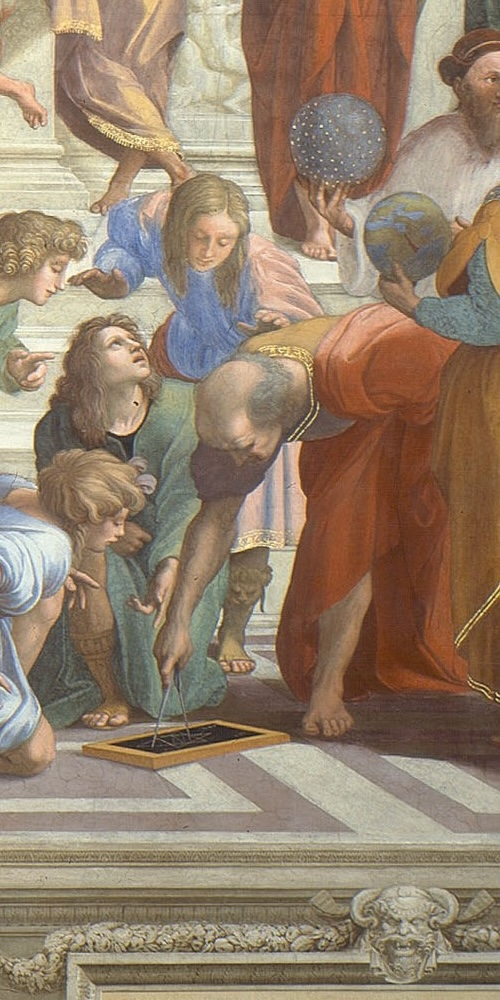
\includegraphics[width=\textwidth]{../graphics/Euclid.jpg}
    \end{center}
\end{columns}
\end{frame}

\appendix
\begin{frame}[plain]
\hspace{0pt}
\vfill
\begin{center}
  \Huge Grazie per l'attenzione
\end{center}
\vfill
\hspace{0pt}
\end{frame}

\end{document}